\section{Comparison with Kira}
\label{sec:cost-comparison}
A useful learned choice must reduce the cost of obtaining the final
master coefficients. The sufficiency test in
Section~\ref{sec:seed-kira-sufficiency} establishes which stored seed
sets permit a reduction, while the preceding target-row test measures
individual reduction paths. We now compare complete symbolic reductions
with Kira's existing equation selection and seeding. The comparisons
retain both trained models, the held-out families and the seed
threshold of one half. The candidate seed lists and prescribed
master bases are inputs; their earlier construction is outside
the measured reduction costs.

\subsection{Targets, baselines and exact checks}
We use 19 held-out family instances: one restricted vacuum profile
at each loop order from one through twelve, three box profiles,
and one bubble, triangle, tadpole and two-loop propagator family.
The three box profiles represent the smallest, middle and largest
candidate-pool sizes in that domain. A fixed hash order selects the
other profiles and the target expressions without consulting previous
model outcomes. Nested batches contain 1, 4 and 16 targets, with
batches of 1 and 3 for the three-target tadpole family.
This gives 56 batch cases and 291 distinct targets.
The restricted vacuum profiles retain the dependent denominators
described in Section~\ref{sec:higher-loop-generation}; their loop orders
do not represent the complexity of general multiloop scattering.

For the supplied-equation comparison, Kira receives the connected
part of the complete stored source pool and applies its own
equation selection, forward elimination and back substitution.
The learned seed method takes the union of the predicted seed sets
for the requested batch and supplies the corresponding stored
IBP identities together with the same background identities.
If any target retains an integral outside the prescribed master
basis, the method reruns the batch with the complete pool.
Both attempts contribute to its cost. This comparison isolates
selection from a common source library; generating that library
is outside these timings.

For the row comparison, the learned model chooses source identities
using a fixed finite-field sample, while
Eq.~\eqref{eq:reduction-action} updates the target coefficients
symbolically in $\mathbb K=\mathbb Q(\boldsymbol x,d)$.
Kira then reduces any remaining terms. A second version applies the
local rule from Section~\ref{sec:reduction-test} through the same
symbolic procedure. This control identifies the cost of the learned
choice relative to the local choice. Both methods retain fixed
source identities and a changing target row, which is the procedure
covered by the training data.

We compare each final coefficient with its constructed rational
reference and independently evaluate the coefficients and saved
row operations at three finite-field points. The physical master
coefficients remain present throughout this experiment.
A reported completion therefore includes the full symbolic target
expansion and its checks. Each batch-method pair runs three times
on the same compute node, with the execution order rotated.
Kira and the model each use one computation thread. At most two
trials run concurrently on the cluster.

\subsection{Learned seed bounds in native Kira}
The seven families with independent propagator bases also permit
native Kira equation generation. Kira reduces the component integrals,
and its exact algebra combines their results into the requested target
expressions. We record generation and reduction separately from this
final combination. Native equation counts refer to the component
reduction; the later combination has separate counts and contributes
to every reported total time. For the default baseline, the seeding bounds are
one above the largest values of $r$ and $s$ among the target components
and prescribed masters. The restricted baseline also bounds
$n_{\rm dot}$ one above its largest required value and uses Kira's
subsector truncation with $l=N-s_{\max}$, where $N$ is the number
of propagators. A third control sets $r$, $s$ and $n_{\rm dot}$ directly to the
largest target/master values, uses the same subsector truncation,
and falls back to the default bounds if needed. Both this control
and the learned method reserve 60 seconds for the first native attempt
and 100 seconds for its fallback, within the complete 180-second limit.
These fixed settings retain Kira's own symmetry
handling and equation selection~\cite{Kira3}; they do not represent
an exhaustive search over its settings.

To apply the seed model before native equation generation, let
$\widehat{\mathcal S}_S$ be the predicted seeds in sector $S$.
For every nonempty set, we pass the bounds
\begin{equation}
 \begin{aligned}
 r_S&=\max_{\boldsymbol\sigma\in\widehat{\mathcal S}_S}r(\boldsymbol\sigma),
 &s_S&=\max_{\boldsymbol\sigma\in\widehat{\mathcal S}_S}s(\boldsymbol\sigma),\\
 n_{{\rm dot},S}
 &=\max_{\boldsymbol\sigma\in\widehat{\mathcal S}_S}
           n_{\rm dot}(\boldsymbol\sigma).
 \end{aligned}
 \label{eq:native-learned-bounds}
\end{equation}
to Kira. These bounds enclose the selected seeds, and Kira can generate
additional seeds within the bounds and inherited subsectors.
Its own generated and selected equation counts therefore measure
the resulting work. An incomplete first attempt triggers the default
native bounds. This direct comparison repeats all four native
methods on the largest fixed target batch in each of the seven
families, giving 99 distinct targets and 84 trials. The learned
method uses the same model and threshold as the supplied-pool test.

\subsection{Measured cost and results}
We record the complete elapsed time from process start to a checked
result. It includes input loading, model loading, feature preparation,
inference, exact algebra, any fallback, coefficient checks and output.
We also record the time with the family already loaded and the model
ready for use. This second quantity represents repeated use of prepared
inputs; the complete process time retains the cost of starting the model.
For a matched case, we compare the median of the three repeats and
define
\begin{equation}
 \rho_T=\frac{\operatorname{median}T_{\rm learned}}
              {\operatorname{median}T_{\rm baseline}}.
 \label{eq:cost-ratio}
\end{equation}
Thus $\rho_T<1$ indicates a lower measured time for that case.
Aggregate ratios use the geometric mean of the paired case ratios.
Trials that reach their time or memory limit remain in the completion
counts and are excluded from ratios that require two completed results.

We distinguish supplied equations, equations selected by Kira,
logged forward insertions and coefficient-field operations.
For a committed target-row step with $n_q$ nonzero source entries,
the last count is $1+2n_q$, as in
Section~\ref{sec:reduction-model}. Feature construction also performs
trial updates of candidate rows. These counts do not measure the
internal polynomial work needed to simplify a rational coefficient.
Runtime includes that work. Memory is the largest sampled sum of
resident process memory for the driver, Kira and its algebra process;
the sampling interval is 50 ms, and shared pages can contribute to
more than one process's count. Every trial has a 180-second limit,
a 1.5 GiB address-space limit per process and a 32 MiB scratch limit.
The comparisons use the existing symbolic Kira~3.1 build with Fermat.
They do not benchmark finite-field reconstruction.

The main comparison contains 792 trials. The full stored-pool
baseline completed 168/168, learned seeds completed 168/168,
learned rows completed 168/168, and local-rule rows completed
168/168. On the 56 completed matched batch cases,
learned seed selection gave complete-process and prepared-input time
ratios of 1.720 and 1.116, respectively. It used the full-pool fallback
in 24 trials.
Across those batches, its supplied source-equation count, including
fallback, was 0.251 times the baseline count, while the
number of equations selected by Kira was 1.027 times
the baseline. The distinction shows how Kira's existing selection
changes the work left after an external seed choice.
The learned method had lower complete-process median time in
0 of 56 batches and lower prepared-input
median time in 15 of 56 batches.

The learned row procedure gave time ratios of 1.719 and 1.205
against the full stored-pool baseline over 56 matched
cases. Its ratios against the local row rule were 1.520 and 1.043.
Before the final Kira call, the learned row procedure completed every
target in 54 of the 56 batches, while the local rule did
so in 55. Kira completed the remaining terms in the
other batches.
For the 53 batch cases in which both row procedures themselves
finished all targets before the final Kira call, their summed
committed coefficient-operation counts were 19,401 and
18,881, giving a ratio of 1.028.
This comparison excludes paths that left part of the reduction to
Kira. The elapsed-time measurements retain all of that later work,
as well as candidate feature preparation and exact coefficient
simplification~\cite{KiraCostComparisonData}.

Kira's own equation selection removes much of the redundant input
in the full-pool baseline. The learned seed filter reduces the
supplied pool, and its measured complete cost includes the added
model work and every fallback. Both learned methods have aggregate
complete-process and prepared-input ratios above one in this
comparison. The row-operation ratio also exceeds one relative to the
local rule on the matched complete preprocessing paths. These results
identify added cost in the current implementations and give no
aggregate reduction in the stated time or committed-operation measures.


\begin{figure}[!htbp]
\centering
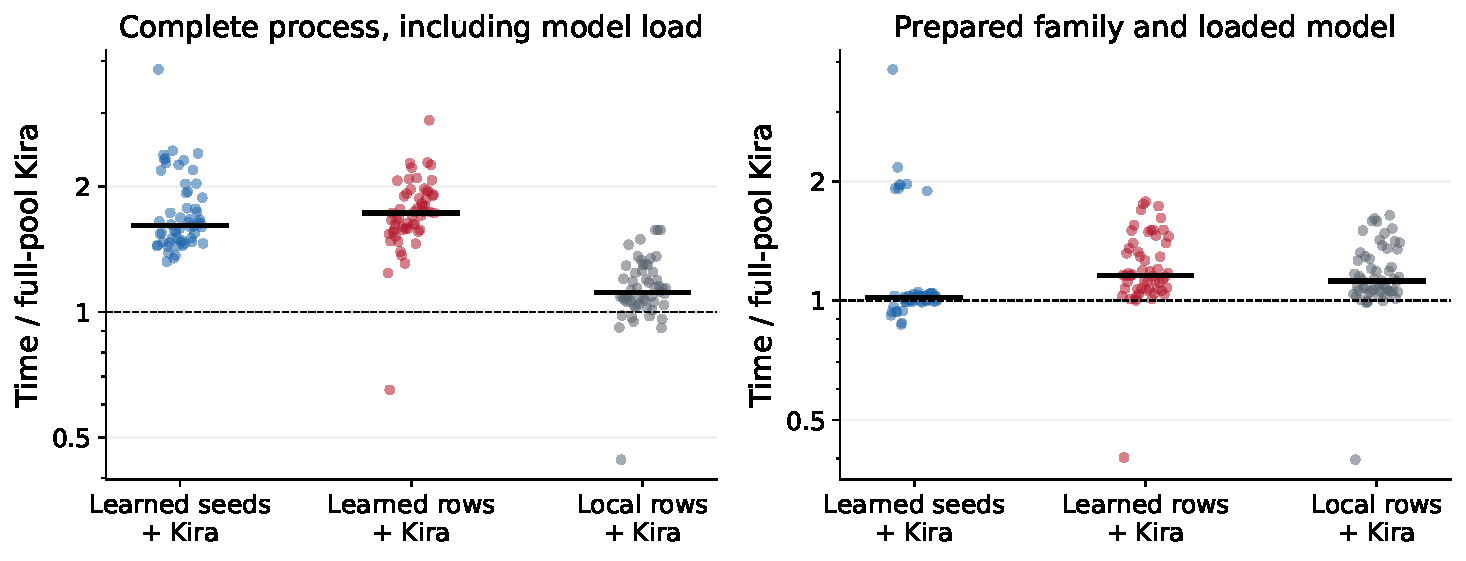
\includegraphics[width=\linewidth]{figures/kira_comparison_time.pdf}
\caption{Matched time ratios relative to Kira with the full stored source pool. Each point uses a batch's three-repeat median. The left panel includes process and model loading; the right panel uses prepared family inputs and a loaded model. Short solid lines show the median case ratio; the dashed line denotes equal time.}
\label{fig:kira-cost-time}
\end{figure}

\begin{figure}[!htbp]
\centering
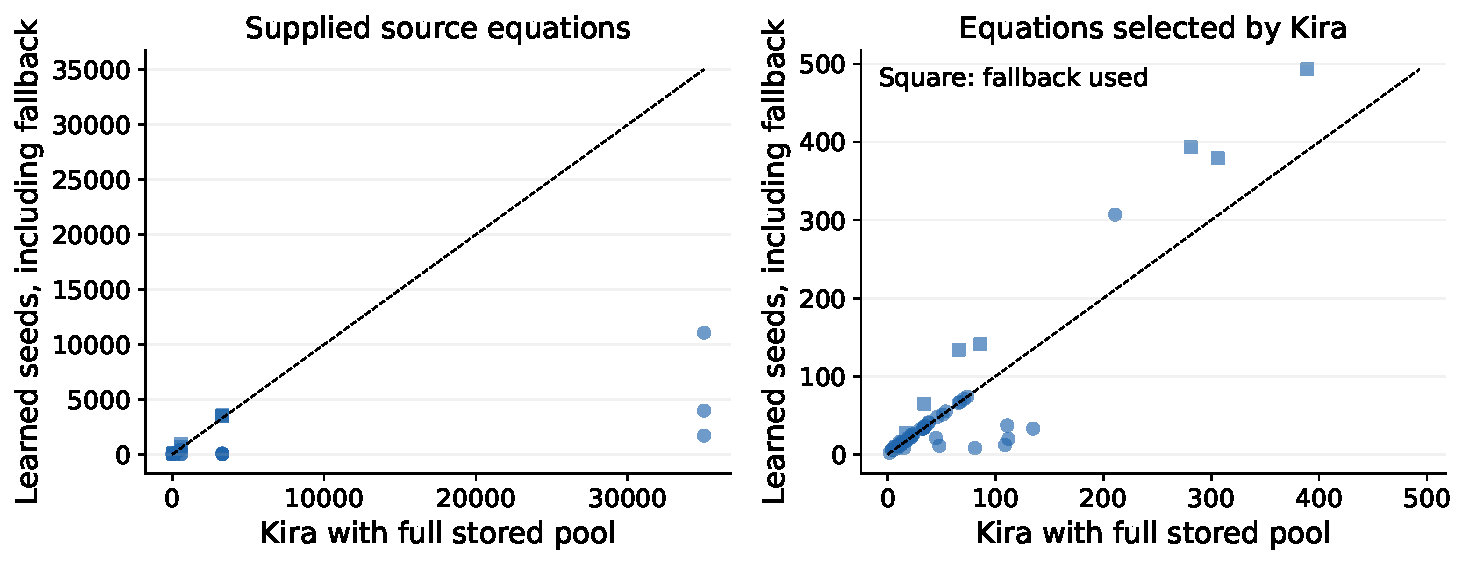
\includegraphics[width=\linewidth]{figures/kira_comparison_equations.pdf}
\caption{Supplied source equations and equations selected by Kira for identical batches. Learned-seed counts include any full-pool fallback. Squares identify batches with fallback, and the diagonal denotes equal counts.}
\label{fig:kira-cost-equations}
\end{figure}

\begin{figure}[!htbp]
\centering
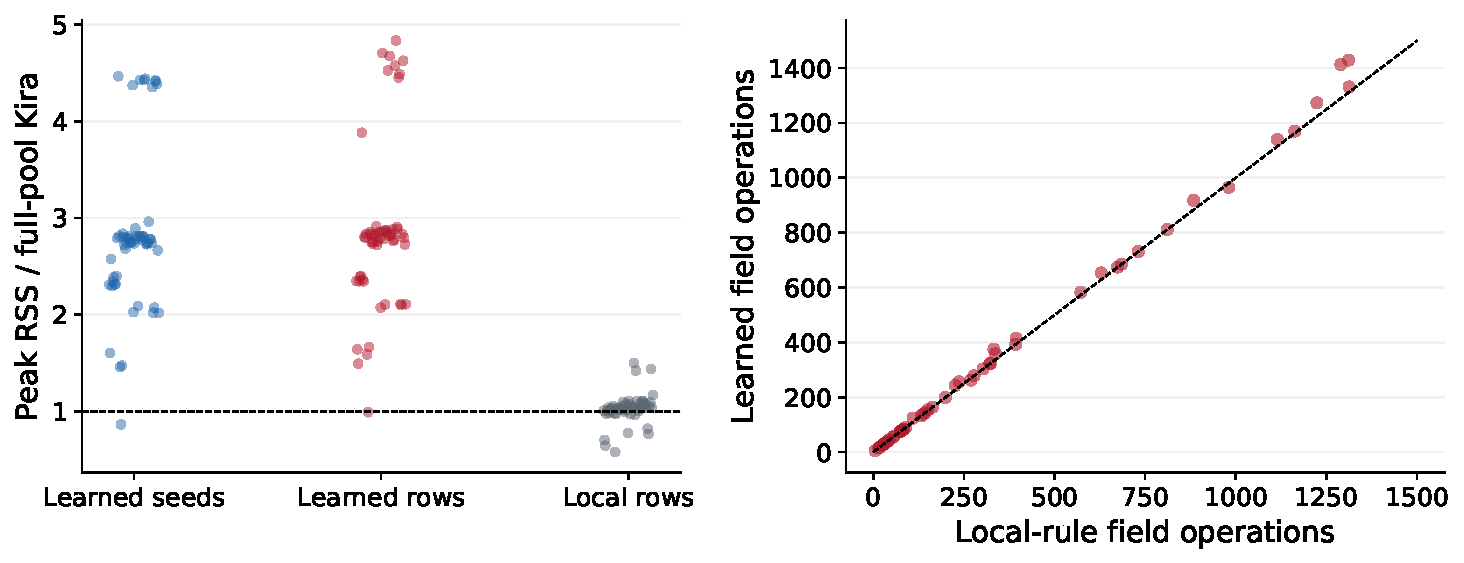
\includegraphics[width=\linewidth]{figures/kira_comparison_memory_operations.pdf}
\caption{Sampled summed resident-memory ratios and committed coefficient-operation counts. Memory ratios use the largest recorded peak within each three-repeat group. The operation panel compares only batches that both row procedures completely reduced before the final Kira call. These counts exclude polynomial simplification and candidate-scoring work.}
\label{fig:kira-cost-memory}
\end{figure}

\FloatBarrier
\subsection{Native seeding results}

The direct native-seeding comparison completed 21/21 learned
trials, 21/21 default-baseline trials, 21/21 restricted-baseline
trials and 21/21 target-index-bound control trials. Learned bounds required a default-bound fallback in
9 trials.
For the 7 paired completed family batches, its
complete-process and prepared-input time ratios against default
native Kira were 1.596 and 1.344. Against restricted native Kira,
the corresponding ratios were 1.671 and 1.373 over 7
paired batches. Against the control that sets bounds directly from target
indices, the ratios were 1.425 and 1.141 over 7 paired batches.
These measurements include native equation
generation, exact reduction, target combination, coefficient checks
and any repeated attempt.

The learned native method had lower complete-process median time
in 0 of 7 matched batches against
the default baseline, 0 of 7 against
the restricted baseline and 1 of 7
against the target-index control. Across the completed paired batches,
the ratios of summed initial equation counts were
0.624,
1.144
and 0.881,
respectively. These counts include repeated attempts.
The learned bounds generate fewer equations than the stated default
bounds, and the restricted deterministic baseline generates still
fewer equations on these batches. The learned method has aggregate
complete-process and prepared-input time ratios above one against
all three native controls. Thus the current native integration adds
total cost under the tested settings.

\begin{figure}[!htbp]
\centering
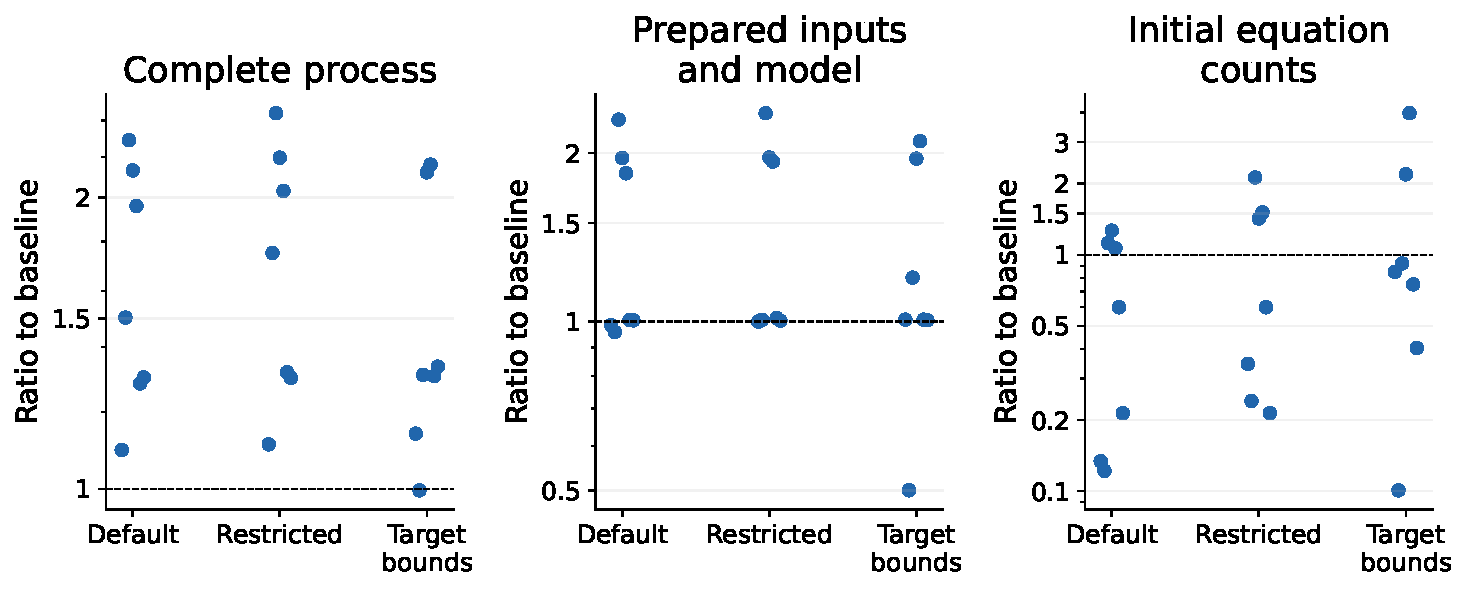
\includegraphics[width=\linewidth]{figures/kira_native_learned_seeds.pdf}
\caption{Direct native-seeding comparison on the largest frozen batches in seven independent-basis families. Ratios compare learned sector bounds with the three stated native baselines. Equation counts sum the initial system sizes that Kira reports for each attempt; internal regeneration can perform additional work.}
\label{fig:native-learned-cost}
\end{figure}

\begin{figure}[!htbp]
\centering
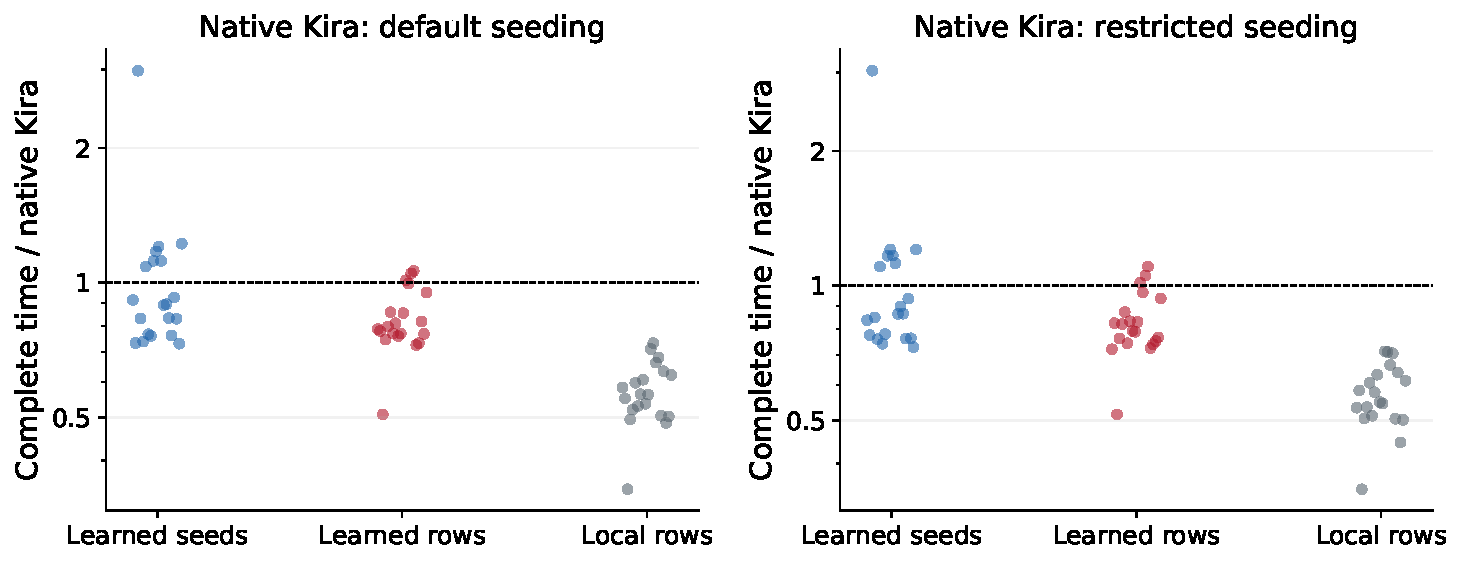
\includegraphics[width=\linewidth]{figures/kira_comparison_native.pdf}
\caption{The methods using stored identities compared with native component reduction at the same targets and master basis. Native timings include equation generation and exact combination of the component results. This comparison changes the available source representation as well as the external method, so it does not isolate the benefit of learning.}
\label{fig:native-stored-cost}
\end{figure}

\FloatBarrier
Across both comparisons, all 876 trials produced a
checked complete result within the stated bounds. The paired timing
ratios above use three completed repeats for both methods.
The recorded limits and three-repeat design bound the interpretation
of small timing differences on the shared cluster.

These results describe the implemented policies and the stated
symbolic Kira settings. The stored-pool tests reuse previously
generated identities, and the native tests measure learned sector
bounds that can include seeds beyond the model's selected set.
The row model acts on fixed source identities and target rows.
A learned policy for every pivot of Kira's evolving matrix, general
high-loop scattering families and finite-field reconstruction
requires further tests. Reduced input counts alone do not establish
a speed improvement because equation selection, model execution,
exact simplification and fallback all contribute to the total cost.
\FloatBarrier
